\documentclass[]{article}
\usepackage{etex}
\usepackage[margin = 1.5in]{geometry}
\setlength{\parindent}{0in}
\usepackage{amsmath}
\usepackage{amsfonts}
\usepackage{amssymb}
\usepackage{amsthm}
\usepackage{bbm}
\usepackage{listings}
\usepackage{color}
\usepackage{mathtools}
\usepackage{multicol}
\usepackage[lined]{algorithm2e}
\usepackage{float}
\usepackage[T1]{fontenc}
\usepackage{ae,aecompl}
\usepackage[pdftex,
  pdfauthor={Michael Noukhovitch},
  pdftitle={COMP767},
  pdfsubject={Lecture notes from Doina Precup},
  pdfproducer={LaTeX},
  pdfcreator={pdflatex}]{hyperref}
\usepackage{graphicx}
\usepackage{cleveref}
\usepackage{enumitem}

\definecolor{dkgreen}{rgb}{0,0.6,0}
\definecolor{gray}{rgb}{0.5,0.5,0.5}
\definecolor{mauve}{rgb}{0.58,0,0.82}

\lstset{
  language=C,
  aboveskip=3mm,
  belowskip=3mm,
  showstringspaces=false,
  columns=flexible,
  basicstyle={\small\ttfamily},
  numbers=none,
  numberstyle=\tiny\color{gray},
  keywordstyle=\color{blue},
  commentstyle=\color{dkgreen},
  stringstyle=\color{mauve},
  breaklines=true,
  breakatwhitespace=true,
  tabsize=4
}

\theoremstyle{definition}
\newtheorem*{defn}{Definition}
\newtheorem{ex}{Example}[section]
\newtheorem*{theorem}{Theorem}

\setlength{\marginparwidth}{1.5in}
\setlength{\algomargin}{0.75em}

\DeclarePairedDelimiter{\set}{\lbrace}{\rbrace}

\definecolor{darkish-blue}{RGB}{25,103,185}

\usepackage{hyperref}
\hypersetup{
    colorlinks,
    citecolor=darkish-blue,
    filecolor=darkish-blue,
    linkcolor=darkish-blue,
    urlcolor=darkish-blue
}
\newcommand{\lecture}[1]{\marginpar{{\footnotesize $\leftarrow$ \underline{#1}}}}
\newcommand{\N}{\mathbb{N}}
\newcommand{\Z}{\mathbb{Z}}
\newcommand{\E}{\mathbb{E}}
\newcommand{\Lagr}{\mathcal{L}}
\newcommand{\ind}{\mathbbm{1}}
\DeclareMathOperator*{\argmin}{argmin}
\DeclareMathOperator*{\argmax}{argmax}

\makeatletter
\def\blfootnote{\gdef\@thefnmark{}\@footnotetext}
\makeatother

\graphicspath{{./comp767/}}

\begin{document}
\let\ref\Cref

\title{\bf{COMP767: Reinforcement Learning}}
\date{Winter 2018, \\ \center Notes written from Doina Precup's lectures, David Silver's online lectures, and Sutton \& Barto 2018 preprint}
\author{Michael Noukhovitch}

\maketitle
\newpage
\tableofcontents
\newpage

\section{Introduction}
\label{sec:introduction}

\subsection{Definitions}
\label{sub:definitions}
Reinforcement learning is:
\begin{description}
    \item[agent-oriented learning] learning by interacting with an environment
    \item[trial and error] only given delayed evaluative feedback
    \item[science of the mind] one which is neither natural science nor applied technology
\end{description}

Framework:
\begin{enumerate}
    \item agent percieves the \textbf{state} of the environment
    \item based on the state, it chooses an \textbf{action}
    \item the action gives the agent a \textbf{reward}
    \item a \textbf{policy} aims to maximize the agent's \textbf{long term expected reward}
\end{enumerate}


\subsection{Key Factors of RL}
\label{sub:key_factors_of_rl}
\begin{itemize}
    \item trial and error search
    \item environment is stochastic
    \item reward may be delayed
    \item balancing exploration and exploitation
\end{itemize}

\subsection{Classical Challenges}
\label{sub:classical_challenges}
\begin{itemize}
    \item reward
    \item information is sequential
    \item delayed consequences
    \item balancing exploration/exploitation
    \item non-stationarity
    \item fleeting nature of time and online data
\end{itemize}


\section{Bandit}
\label{sec:bandit}

\subsection{Definition}
\label{sub:definition}

\textbf{One-armed bandit} Simplest RL problem
\begin{itemize}
    \item pull the lever
    \item get some reward
    \item choose the best lever!
\end{itemize}

\textbf{k-armed bandit} extends to $k$ arms
\begin{itemize}
    \item at every time step $t$, choose an action $A_t$ from $k$ possibilties
    \item recieve a reward $R_t$ dependent only on the action taken (i.i.d)
    \item $q_*(a) = \E [R_t | A_t = a], \medskip \forall a \in {1, \ldots k }$
\end{itemize}

\subsection{Action Selection}
\begin{description}
    \item[greedy] the action with the current highest expected value (best one so far)
    \item[exploitation] choosing the greedy action
    \item[exploration] choosing not the greedy action
    \item[$\varepsilon$-greedy] balance explore/exploit by choosing exploration (random) with probability $\varepsilon$
\end{description}
\begin{figure}[ht]
    \centering
    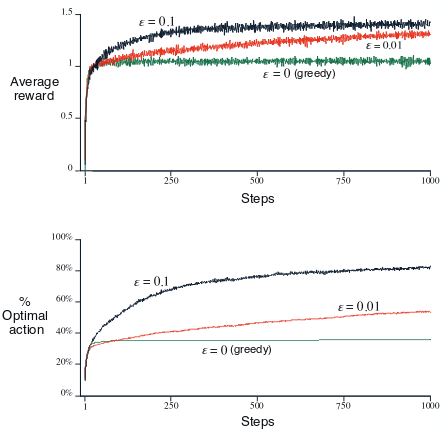
\includegraphics[width=0.5\linewidth]{epsilon_10arm.png}
    \caption{$\epsilon$-greedy methods on 10-arm bandit}
    \label{fig:}
\end{figure}

\subsection{Learning Rules}
\label{sub:learning_rules}

Learn the best policy by learning the reward for an action

\subsubsection{Averaging}
\label{ssub:averaging}

For a single action, update the new estimate based on old estimate and step size ($\alpha$), with all actions being equal
\begin{equation*}
    Q_{n+1} = Q_n + \alpha (R_n - Q_n)
\end{equation*}

\subsubsection{Recency-Weighted Average}
\label{ssub:recency_weighted_average}

\begin{description}
    \item[stationary] if the true action values DO NOT change over time
\end{description}

if our bandit is non-stationary, then we need to put more weight on recent samples
\begin{equation*}
    Q_{n+1} = (1 - \alpha)^n Q_1 + \sum_{i=1}^n \alpha(1 - \alpha)^{n - i} R_i
\end{equation*}

\subsubsection{Optimistic}
\label{ssub:optimistic}
Previously we assumed $Q_1(a) = 0$, but we can start optimistically (e.g. $Q_1(a) = 5$) to encourage early exploration

\subsubsection{Upper Confidence Bound}
\label{ssub:upper_confidence_bound}
Reduce exploration over time after starting confident
\begin{itemize}
    \item estimate upper bound on true action values
    \item select the action with the largest upper bound
\end{itemize}

\begin{equation*}
    A_t = \argmax_a [Q_t(a) + c \sqrt{\frac{\log t}{N_t(a)}}]
\end{equation*}

\subsubsection{Gradient-Bandit Algorithms}
\label{ssub:gradient_bandit_algorithms}

Don't need to learn specific rewards, just learn the \textbf{preference} $H_t(a)$, and try and make the probability of choosing an action $\pi_t(a)$ be proportional to it.

\begin{eqnarray*}
    \pi_t(a) &\propto e^{H_t(a)} \\
             &= \frac{e^{H_t(a)}}{\sum_b e^{H_t(b)}}
\end{eqnarray*}

if the reward for an action is better than average, increase its preference
\begin{eqnarray*}
    H_{t+1} &= H_t(a) + \alpha(R_t - \bar R_t)(1_{a = A_t} - \pi_t(a)) \\
\end{eqnarray*}
where $\bar R_t = $ average $R_i$

\subsubsection{Associative Search}
\label{ssub:associative_search}

\begin{description}
    \item[associative] a task where the situation/state of the agent changes the reward for an action
    \item[contextual bandit] not just trial-and-error search, but also association between state and action values
    \item[full reinforcement learning] trial-and-error search, association between state and action, and actions affecting the next state of the agent
\end{description}


\subsection{Evaluations}
\label{sub:evaluations}
\begin{description}
    \item[regret] the difference between best option and the one we chose $\max_a q_*(a) - q_t(a)$
    \item[expected total regret] $\E[\sum_t $ regret$_t]$ (optimal for UCB, Thomson sampling)
    \item[best response] regret for $T$ experimental trials after policy is fixed
\end{description}

\subsection{Conclusions}
\label{sub:conclusions}
\begin{itemize}
    \item simple methods that can be built on
    \item learn from feedback
    \item appear to have a goal
\end{itemize}

\begin{figure}[ht]
    \centering
    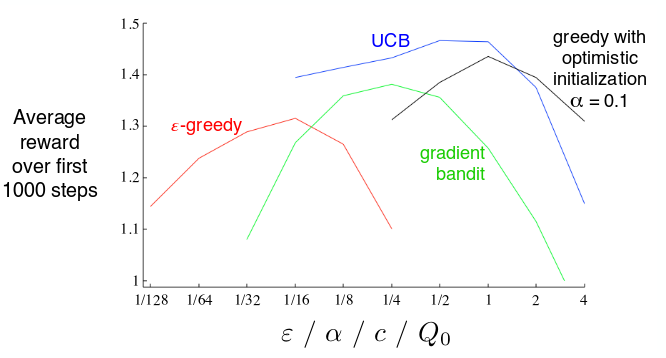
\includegraphics[width=0.7\linewidth]{bandit_comparison.png}
    \caption{bandit algorithm comparison}
    \label{fig:bandit-comparison}
\end{figure}

\section{Markov Decision Processes}
\label{sec:markov_decision_processes}

\subsection{Markov Reward Processes}
\label{sub:markov}

\subsubsection{Markov}
\label{ssub:markov}


\begin{description}
    \item[markov property] future independent of past given present
    \item[markov chain] memoryless random process with states $S$ and transition probs $P$, $<S,P>$

    \item[markov reward process] markov chain with values: rewards $R$, discount factor $\gamma$
    \item[return] sum of discounted rewards $G_t = R_t + \gamma R_{t+1} + \gamma^2 R_{t+2} \ldots$
    \item[value function] long-term value of state $s$, $v(s) = E[G_t | S_t = s]$
\end{description}

\subsubsection{Bellman Equations}
\label{ssub:mrp_bellman_equations}

Breaking value function into present and future
\begin{align*}
    v(s) &= E[G_t | S_t = s] \\
         &= E[R_{t+1} + \gamma v(S_{t+1}) | S_t = s] \\
    v &= R + \gamma P v \\
\end{align*}


\subsection{Markov Decision Processes}
\label{sub:markov_decision_processes}

\subsubsection{Policy}
\label{ssub:policy}

\begin{description}
    \item[markov decision process] MRP with actions $A$
    \item[finite MDP] finite number of states, actions, and rewards
    \item[policy] distribution over actions, given states $\pi (a|s)$
    \item[trajectory] sequence of actions, states, and rewards
\end{description}

\subsubsection{Value Function}
\label{ssub:value_function}

\begin{description}
    \item[state-value function] expected return starting from $s$ following \\
        $\pi$, $v_{\pi}(s) = \E [G_t | S_t = s]$
    \item[action-value function] expected return starting from $s$, taking action $a$, then following $\pi$ \\
        $q_\pi(s,a) = \E_\pi[G_t | S_t =s, A_t = a]$
\end{description}

\subsubsection{Bellman Expectation Equations}
\label{ssub:bellman_expectation_equations}
\begin{align*}
    v_\pi(s) &= \sum_{a \in A} \pi(a|s)q_\pi(s,a) \\
    q_\pi(s,a) &= R_{s}^a + \gamma \sum_{s' \in S} P_{ss'}^a v_\pi(s')
\end{align*}
substitute one into the other to get their Bellman equations, succinctly
\begin{equation}
    v_\pi = R^\pi + \gamma P^\pi v_\pi
\end{equation}

\subsubsection{Optimal Value}
\label{ssub:optimal_value_function}
\begin{description}
    \item[optimal state-value function] maximum value function $v_*(s) = \max_\pi v_\pi(s)$
    \item[optimal action-value function] maximum action-value function $q_*(s) = \max_\pi q_\pi(s,a)$
\end{description}

\subsubsection{Optimal Policy}
\label{ssub:optimal_policy}
\begin{description}
    \item[policy ordering] $\pi \geq \pi' \text{ if } v_\pi(s) \geq v_{\pi'} \ \forall s$
    \item[optimal policy theorem] $\exists $ optimal policy $\pi_* \geq \pi' \ \forall \pi'$ and $v_{\pi_*} = v_*$
\end{description}

\subsubsection{Bellman Optimality Equations}
\label{ssub:bellman_optimality_equations}

\begin{align*}
    v_*(s) &= \max_a q_*(s,a) \\
    q_*(s, a) &= R_s^a + \gamma \sum_{s' \in S} P^a_{ss'} v_*(s')
\end{align*}
no closed form, so solve using iterative solutions

\subsection{Extensions to MDPs}
\label{sub:extensions_to_mdps}

\subsubsection{Infinite MDPs}
\label{ssub:infinite_mdps}
\begin{itemize}
    \item countably infinite states and/or action spaces
    \item continuous states and/or action spaces
    \item continuous time
\end{itemize}

\subsubsection{POMDPs}
\label{ssub:pomdps}

\begin{description}
    \item[POMDP] partially observable MDP, observations $O$, observation function $Z$
    \item[history] sequence of actions, observations, rewards
    \item [belief state] probability dist over states given history $b(h)$
\end{description}

\subsubsection{Average Reward MDP}
\label{ssub:average_reward_mdp}

\begin{description}
    \item [recurrent] each state visited infinite amount of times
    \item [aperiodic] each state visited without any systematic period
    \item [ergodic MC] stationary distribution $d^\pi(s) = \sum_{s' \in S} d^\pi(s')P_{s's}$
    \item [ergodic MDP] if some MC induced by a policy is ergodic, uses \textit{average reward} $\rho$ \\
        \begin{align*}
            \rho^\pi &= \lim_{T \to \infty} \frac{1}{T} \E [\sum_{t=1}^T R_t] \\
            \tilde v_\pi(s) &= \E_\pi [\sum_{k=1}^\infty (R_{t+k} - \rho^\pi) | S_ts = s] \\
                            &= \E_\pi [R_{t+1} - \rho^\pi)  + \tilde v_\pi(S_{t+1}| S_ts = s]
        \end{align*}
\end{description}


\section{Dynamic Programming}
\label{sec:dynamic_programming}

\subsection{Introduction}
\label{sub:introduction}

\begin{description}
    \item[dynamic programming] solving problems by breaking down into subproblems
    \item [optimal substructure] subproblems solve a larger problem
    \item [overlapping subproblems] subproblems recur many times
\end{description}

used either for
\begin{itemize}
    \item planning: MDP and policy $\to$ value function
    \item control: MDP $\to$ optimal value function, optimal policy
\end{itemize}

\subsection{Policy Evalutation}
\label{sub:policy_evalutation}

\subsubsection{Iterative Policy Evaluation}
\label{ssub:someting}

\begin{description}
    \item[synchronous backups] iterative evaluation of $\pi$ using Bellman
\end{description}
\begin{equation*}
    v^{k+1} = R^\pi + \gamma P^\pi v^k
\end{equation*}
\begin{itemize}
    \item update $v_{k+1}(s)$ from $v_k(s')$
    \item for iteration $k+1$
    \item for all states $s \in S$
    \item where $s'$ is successor state of $s$
\end{itemize}


\subsection{Policy Iteration}
\label{sec:policy_iteration}

\subsubsection{Policy Iteration Basics}%
\label{ssub:policy_iteration_basics}
\begin{enumerate}
    \item evaluate the policy with \textbf{Bellman Expectation}, estimate $v_\pi$
    \item improve the policy \textbf{greedily}, generate $\pi' \geq \pi$
\end{enumerate}
always converges to optimal policy $\pi_*$

\subsubsection{Convergence}
\label{ssub:convergence}
convergence when policy no longer improves
\begin{align*}
    v_\pi(s) &= v_{\pi'}(s) \\
             &= \max_{a \in A} q_\pi(s,a) \\
    \intertext{is the bellman optimality equation, $\pi = \pi_* \qed$}
\end{align*}

\subsubsection{Modified Policy Iteration}%
\label{ssub:modified_policy_iteration}
achieve optimal policy without fully converging

\begin{description}
    \item[$\epsilon$-convergence] converge after no more than $\epsilon$ change
    \item[$k$-iterations] just stop after $k$
\end{description}

\subsection{Value Iteration}
\label{sub:value_iteration}

\subsubsection{Principle of Optimality}%
\label{ssub:principle_of_optimality}

A policy $\pi(a|s)$ achieves optimal value at $s$ iff it achieves optimal value at any successor state $s$

\subsubsection{Value Iteration}%
\label{ssub:value_iteration}
\begin{figure}[htpb]
    \centering
    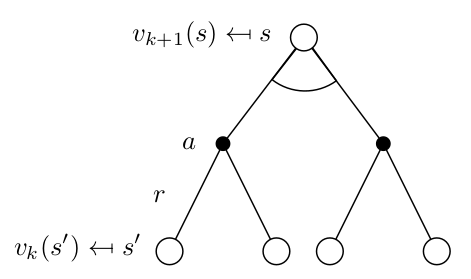
\includegraphics[width=0.5\linewidth]{value-iteration.png}
    \caption{value-iteration}
    \label{fig:value-iteration}
\end{figure}
\textbf{Bellman Optimality Backup}, iteratively
\begin{equation*}
    v_{k+1} \gets \max_{a \in A} R^a + \gamma P^a v_k
\end{equation*}
always converges to optimal value $v_*$

\subsection{Extensions to DP}
\label{sub:extensions_to_dp}

\begin{description}
    \item[asynchronous DP] back up states individually in any order
    \item[in-place DP] don't store $v_{old}$ only keep updated value function
    \item[prioritized sweeping] update states based on their magnitude of Bellman error
    \item[real time DP] only update states that agent actually visits
    \item[sample backups] break curse of dimensionality by sampling instead of full backup
    \item[approximate DP] approximate the value function $\hat v(s, w_k)$ \\
        train new $\hat v(s, w_{k+1})$ on results of optimality backup $s \to Bellman(\hat v(s, w_k))$
\end{description}

\subsection{Contraction Mapping}
\label{sub:contraction_mapping}

\begin{description}
    \item[contraction mapping theorem] for any metric space $V$, complete under operator $T(v)$, where $T$ is a $\gamma$-contraction then $T$ converges to a fixed point at rate $\gamma$
\end{description}
\begin{align*}
    \intertext{Bellman Backup}
    T^\pi(v) &= R^\pi + \gamma P^\pi v \\
    ||T^\pi(u) - T^\pi(v)||_\infty &= ||R^\pi + \gamma P^\pi u  - R^\pi + \gamma P^\pi v ||_\infty
                                   &= ||\gamma P^\pi (u - v)||_\infty \\
                                   &\leq ||\gamma P^\pi ||u - v||_\infty ||_\infty \\
                                   &\leq \gamma||u - v||_\infty
    \intertext{so $T(v)$ is a $\gamma$-contraction}
\end{align*}

\section{Model-Free Prediction}
\label{sec:model_free_prediction}

\begin{description}
    \item[model-free prediction] estimate the value function of an unknown MDP
\end{description}

\subsection{Monte-Carlo Learning}%
\label{sub:monte_carlo_learning}

\begin{description}
    \item[MC learning] sample complete episodes using value = mean return
    \item[sampling] update samples an expectation
\end{description}


\subsubsection{MC Policy Evaluation}
\label{ssub:mc_policy_evaluation}
learn $v_\pi$ from episodes under $\pi$, using the average of the return after visiting state $s$
\begin{description}
    \item[every visit MC] average returns for every visit to $s$
    \item[first visit MC] average returns for only the first visit to $s$ (in an episode)
\end{description}

\subsubsection{Incremental Monte-Carlo}%
\label{ssub:incremental_monte_carlo}
the mean of a sequence can be computed incrementally
\begin{equation*}
    \mu_k = \mu_{k-1} + \frac{1}{k}(x_k + \mu_{k-1})
\end{equation*}
so we can make our MC updates incremental, and use constant step size $\alpha$
\begin{equation*}
    V(S_t) \gets V(S_t) + \alpha (G_t - V(S_t))
\end{equation*}

\subsection{Temporal Difference Learning}%
\label{sub:temporal_difference_learning}

\subsubsection{Basic TD}%
\label{ssub:basic_td}
\begin{description}
    \item[TD learning] update value function towards estimated return, bootstrapping
    \item[bootstrapping] update involves an estimate
\end{description}
For basic TD(0)
\begin{description}
    \item[TD target] estimated return $R_{t+1} + \gamma V(S_{t+1})$
    \item[TD error] actual - estimated $R_{t+1} + \gamma V(S_{t+1}) - V(S_t)$
\end{description}

\begin{equation*}
    V(S_t) \gets V(S_t) + \alpha(R_{t+1} + \gamma V(S_{t+1}) - V(S_t))
\end{equation*}

\subsubsection{Advantages of TD vs MC}%
\label{ssub:advantages_of_td}

\begin{itemize}
    \item learn before knowing the final outcome
        \begin{itemize}
            \item learn online after every step
        \end{itemize}
    \item learn without the final outcome
        \begin{itemize}
            \item learn from incomplete/non-terminating sequences
        \end{itemize}
    \item low variance, some bias (vs. high variance, no bias)
        \begin{itemize}
            \item more efficient
            \item more sensitive to initial value
            \item also converges (except w/ function approximation)
        \end{itemize}
    \item exploits the Markov property
        \begin{itemize}
            \item optimizes for max-likelihood Markov model
            \item more effective in Markov environments
        \end{itemize}
\end{itemize}

\subsubsection{Unified View}%
\label{ssub:unified_view}

\begin{figure}[ht]
    \centering
    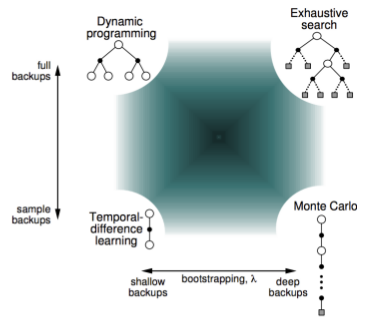
\includegraphics[width=0.5\linewidth]{unified-view.png}
    \caption{unified view of RL}
    \label{fig:unified-view}
\end{figure}

\subsection{TD-$\lambda$}%
\label{sub:td_lambda_}

\subsubsection{$n$-step TD}%
\label{ssub:_n_step_td}

\begin{description}
    \item[TD$(n)$] extension of TD to deeper, $n$-step backups
    \item[online update] immediately update value function
    \item[offline update] update value function at end of episode
\end{description}
\begin{align*}
    G_t^{(n)} &= R_{t+1} + \gamma R_{t+2} + \ldots + \gamma^n V(S_{t+n}) \\
    V(S_t) &\gets V(S_t) + \alpha (G_t^{(n)} - V(S_t))
\end{align*}

\subsubsection{TD-$\lambda$}%
\label{ssub:averaging_n_step_returns}
\begin{description}
    \item[TD-$\lambda$] use factor $\lambda$ to combine all n-step returns
\end{description}

\begin{align*}
    G_t^{\lambda} &= (1 - \lambda) \sum_{n=1}^\infty \lambda^{n-1} G_t^{(n)} \\
    V(S_t) &\gets V(S_t) + \alpha (G_t^\lambda - V(S_t))
\end{align*}

\subsubsection{Eligibility Traces}%
\label{ssub:eligibility_traces}
\begin{description}
    \item[frequency heuristic] assign credit to most frequent states
    \item[recency heuristic] assign credit to most recent states
    \item[eligibility trace] combine both, $E_t(s) = \gamma \lambda E_{t-1}(s) + \mathbbm{1} (S_t = s)$
\end{description}

\subsubsection{Backward-View TD-$\lambda$}%
\label{ssub:backward-view}

\begin{description}
    \item[forward-view] look into future to compute $G_t^\lambda$
        \begin{itemize}
            \item offline, has to wait until end of episode
        \end{itemize}
    \item[backward-view] look into past and compute for any sequence, online
        \begin{itemize}
            \item keep eligibility trace for every state
            \item update value in proportion to eligibility trace $E_t(S)$ and TD-error $\delta_t$
        \end{itemize}
\end{description}
\begin{align*}
    \delta_t &= R_{t+1} + \gamma V(S_{t+1}) - V(S_t) \\
    V(S_t) &\gets V(S) + \alpha \delta_t E_t(s)
\end{align*}

\subsection{Summary}%
\label{sub:summary}

\begin{figure}[ht]
    \centering
    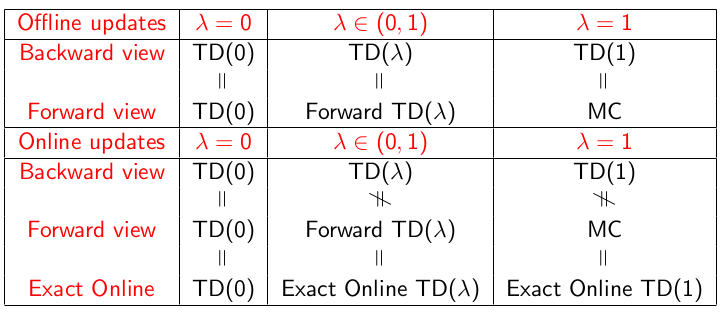
\includegraphics[width=0.5\linewidth]{td-lambda-summary.png}
    \caption{TD-$\lambda$ summary}
    \label{fig:td-lambda-summary}
\end{figure}

\section{Value Function Approximation}%
\label{sec:value_function_approximation}

\subsection{Introduction}%
\label{sub:introduction}

\subsection{Incremental Methods}%
\label{sub:_incremental_methods}

\subsection{Batch Methods}%
\label{sub:batch_methods}

\subsubsection{Linear Least Squares Prediction}%
\label{ssub:linear_least_squares_prediction}

$\hat v(s,w) = x(s)^Tw$
\begin{itemize}
    \item sidenote: we want feature vectors $x \in X$ where $X^TX$ is full rank
\end{itemize}

\begin{align*}
    \intertext{since the expected update is 0}
    E_D[\Delta w] &= 0 \\
    ...
\end{align*}

but since we don't know $v^\pi_t$
\begin{description}
    \item[LS Monte Carlo] $v^\pi_t \approx G_t$
    \item[LS TD] $v^\pi_t \approx R_{t+1} + \gamma \hat v(S_{t+1},w)$
    \item[LS TD($\lambda$)] $v^\pi_t \approx G_t^\lambda$
\end{description}

\subsubsection{Least Squares Control}%
\label{ssub:least_squares_control}
\textbf{LS policy iteration}
\begin{itemize}
    \item policy evaluation with LS Q-learning
    \item greedy policy improvement
\end{itemize}
\textbf{LS Q-learning} approximate $q_\pi(s,a) \approx \hat q(s,a,w) = x(s,a)^T w$
\begin{itemize}
    \item must learn off policy
\end{itemize}




%\subsection{On-Policy MC Control}
%\label{sub:on_policy_mc_control}

%\begin{description}
    %\item[on policy] learn about policy currently executing
    %\item[boltzmann exploration] choose with probability $\exp (- \frac{P(s)}{T} )$ where $T$ is a temperature.  \\
        %Over time, decrease from high $T$ (equiprobable) to low $T$ (biased towards best action)
%\end{description}

%\subsection{Advantages}
%\label{sub:advantages}
%Several advantages over DP
%\begin{itemize}
    %\item can learn directly from interaction with environment
    %\item no need for full models
    %\item no need to learn about all states
    %\item less harmed by violating Markov property
%\end{itemize}


\section{Temporal Abstraction}
\label{sec:temporal}
Overview of \textit{Between MDPs and semi-MDPs: A framework for temporal abstraction in reinforcement learning} (Sutton, Precup, Singh 1999)

\subsection{Options Framework}
\label{sub:options_framework}

\subsubsection{Definition}
\label{ssub:definition}
\textbf{Options} an MDP over an augmented state space
\begin{enumerate}
    \item initiation set $I_o$
    \item policy for that option $\pi_o$
    \item termination condition $\beta_o$
\end{enumerate}

\subsubsection{Options}
\label{ssub:options}
a set of options and a policy induces a Semi-MDP

\subsubsection{Bellman Equations}
\label{ssub:options_bellman_equations}

\begin{align*}
    q(s,o) &= \sum_a \pi_o (a,s) (r(s,a) + )   \\
    u(s',o) & = (1 - \beta_o(s')) q(s', o) + \Beta_o(s') \sum_{o'} \mu (o'|s')q(s',o') &\\
    &= q(s',o) - \beta_o(s')(q(s',o) - v(s')) \\
    &= q(s',o) - \beta_o(s')A(s',o) \\
\end{align*}

\subsection{Intra-Option Value Learning}
\label{sub:intra_option_value_learning}

derive TD-style algorithm in a similar way
\begin{equation}
    q(S_t, O_t) = q(S
\end{equation}

\subsection{Option Models}
\label{sub:option_models}

\subsubsection{Bellman Equations}
\label{ssub:option_model_bellman_equations}

\subsubsection{Bellman Equations at SMDP level}
\label{ssub:bellman_equations_at_smdp_level}
everything behaves like an MDP over transformed reward and transition functions/models


\subsubsection{TD at SMDP level}
\label{ssub:td_at_smdp_level}

\end{document}
